%&latex
\chapter{Introduzione}
In questo testo viene illustrata una procedura semplice per l'installazione di \textit{Debian 8 "jessie"}, una delle distribuzioni più utilizzate al mondo.

Questo documento, che fa parte del progetto \textbf{Hacklog} promosso dalla comunità di \textbf{inforge.net}, è rilasciato sotto licenza \texttt{Creative Commons}, il codice sorgente \LaTeX{} è liberamente fruibile all'indirizzo:

\begin{graybox}
	\texttt{https://github.com/InforgeNet/hacklog-debian}
\end{graybox}

Inizieremo prima con una breve introduzione a Linux e a Debian.
%&pdflatex
\section{Parliamo di Linux}
Linux è un sistema operativo \textit{libero} e \textit{open-source}: il codice è liberamente disponibile e chiunque può vederlo e modificarlo (il codice è disponibile su \texttt{kernel.org}). La prima versione del \textit{kernel} Linux (il kernel è il programma del sistema operativo che gestisce l'hardware e le sue risorse e viene avviato per primo con all'accensione del computer, subito dopo il software di \textit{bootstrap}) è la \(0.01\) e risale al 1991. È stato sviluppato da Linus Torvalds. Ad oggi esistono numerose \textit{distribuzioni Linux}, ossia sistemi Linux con software preinstallato e configurato.

Gran parte del software di base disponibile in tutte le distribuzioni Linux fa parte del progetto \textit{GNU}, fondato da Richard Stallman (si veda \texttt{www.gnu.org}). Talvolta si parla infatti di \textit{distribuzioni GNU/Linux}.

Linux è uno dei sistemi operativi più utilizzati al mondo: domina nel mercato mobile con Android (il kernel di Android è Linux); nel mondo dei server e dei supercomputer; e nei \textit{sistemi embedded}. Per quanto non abbia il dominio dei sistemi Desktop (dove spopola \textit{Microsoft Windows}) è comunque molto diffuso.

Si dice talvolta che Linux sia solo per le persone esperte, o che sia utile a svolgere soltanto alcuni compiti specifici. In realtà ciò è falso: \textbf{Linux è per tutti}. Linux è, per molti aspetti, anche molto più facile da utilizzare rispetto a Windows o ad altri sistemi. Ciò che fa sembrare Linux complicato è l'abitudine ad un altro sistema operativo, come appunto a Windows. Ma Linux è diverso da Windows, funziona in modo diverso, e va usato in modo diverso. Se si cerca di utilizzare Linux come si utilizza Windows, inevitabilmente si finirà per fallire, e per ritenerlo erroneamente un sistema operativo complicato. Consideriamo un esempio:

In Linux esistono dei grandi \textit{database} di software, chiamati \textbf{repository}, dai quali l'utente può scaricare tutti i programmi di cui ha bisogno. I repository esistono anche nel mobile, e i pochi lettori di questo documento probabilmente li usano tutti i giorni senza saperlo: il \texttt{Play Store} è il repository di Android; l'\texttt{App Store} è il repository di iOS per iPhone e iPad. Quindi in Linux, si può dire, il software si installa come si installerebbe su uno smartphone: da un'app dedicata che funziona da \textit{shop}.

In Windows funziona in un altro modo: il software va scaricato dal web e installato. Per installare un software su Windows bisogna seguire questi passaggi:
\begin{enumerate}
	\item Cercare su Google (o un altro motore di ricerca) il nome del programma;
	\item Scegliere il sito giusto (altrimenti \textit{malware} e \textit{virus} a volontà!);
	\item Navigare in mezzo al sito pieno di pubblicità per trovare il download;
	\item Scaricare l'\textit{installer};
	\item Avviare l'installer;
	\item Disattivare tutta la pubblicità e il software che non si desidera dall'installer;
	\item Configurare l'installazione (Avanti, Avanti, Avanti, \ldots);
	\item Installare.
\end{enumerate}
In Linux, invece (presentiamo un esempio con Debian, in altre distribuzioni può essere leggermente diverso), per installare un programma è sufficiente:
\begin{enumerate}
	\item Scrivere nel terminale: \texttt{apt-get install \textit{nome-prog}}
\end{enumerate}
Fine. Tutto qui. Le persone, quando provano Linux, finiscono spesso per tentare di installare programmi scaricandoli dal web. Siccome non ci riescono (perché questo non è il modo in cui in Linux si scaricano e si installano i programmi) allora finiscono per tornare su Windows pensando che Linux sia complicato. Ma Linux non è complicato, anzi è pure più semplice (un solo passaggio contro otto passaggi) --- però è \textit{diverso}.

È normale incontrare difficoltà all'inizio con Linux: questione di abitudine, il lettore non si scoraggi alla prima difficoltà.

%&pdflatex
\section{Debian GNU/Linux}
\textbf{Debian} è il principale argomento di questo testo. In questo paragrafo vediamo le caratteristiche distintive di questa distribuzione GNU/Linux.

Intanto, come abbiamo già detto, il fatto che sia una distribuzione \textit{GNU/Linux} ci dice che Debian ha come kernel Linux e contiene i software GNU. Di seguito sono elencate alcune delle caratteristiche che distinguono questa distribuzione:
\begin{itemize}
	\item Debian è composta unicamente da \textit{software libero}: significa che l'utente ha la libertà di eseguire, copiare, distribuire, studiare, modificare e migliorare il software;
	\item I repository di Debian contengono oltre \(43\,000\) pacchetti software;
	\item Nel tempo sono state rilasciate varie versioni di Debian: attualmente Debian è alla \textit{versione 8.6 "jessie"};
	\item Debian usa il software \texttt{apt} per gli aggiornamenti. Segue una politica di aggiornamento standard sul modello \textit{"release cycle"}. Ciò significa che tutto il software di Debian è stato preventivamente testato a lungo al fine di risolvere bug e problemi; inoltre Debian aggiorna il software per includere nuove \textit{feature} soltanto quando rilascia una nuova versione dell'intera distribuzione Debian (fix di sicurezza e bug sono sempre rilasciati il prima possibile). Vuol dire che, ad esempio, il software non viene aggiornato in Debian 8 finché non verrà rilasciata Debian 9. Questa politica serve a garantire maggior stabilità. La politica complementare si chiama \textit{"rolling release"} dove il software viene sempre aggiornato il prima possibile all'ultima versione (\textit{ArchLinux} e \textit{Gentoo} sono esempi di distribuzioni rolling);
	\item Debian usa \texttt{systemd} come \textit{init system}. L'init system è il primo programma che viene avviato su una qualsiasi distribuzione Linux: si occupa di inizializzare tutti i \textit{demoni} (programmi in background) e resta in esecuzione fino allo spegnimento del sistema. Conoscere il proprio init system è fondamentale per chiunque voglia imparare davvero a lavorare bene con un sistema Linux. \texttt{systemd} in realtà è anche molto più che un semplice init system e gestisce vari aspetti del sistema operativo --- viene criticato da una parte della comunità di Linux e del software libero (tra cui anche Linus Torvalds, Patrick Volkerding, Eric Raymond e l'autore di questo documento \texttt{:P}) per alcune scelte di design: log binari; violazione della filosofia Unix; \textit{feature creeping}; ecc\ldots. \texttt{systemd} è l'init system più diffuso;
	\item Da Debian derivano quasi tutte le altre distribuzioni Linux: Debian è, in un certo senso, la distribuzione padre di tutte le altre.
\end{itemize}
Per maggiori informazioni su Debian si veda \texttt{www.debian.org} e \texttt{en.wikipedia.org/wiki/Debian}.
%&pdflatex
\subsection{Ottenere Debian 8 "jessie"}
Ogni versione Debian ha un \textit{nome in codice}: quello di Debian 8 è \textit{"jessie"}. Attualmente Debian 8 è l'ultima versione disponibile. Quando sarà rilasciata, Debian 9 si chiamerà \textit{"stretch"} --- al momento in \textit{testing}. In quanto segue tratteremo solo \textbf{Debian 8 "jessie"}: nel caso che Debian 9 (o una versione ancora più recente) sia stata rilasciata come \textit{stable}, il lettore è invitato a scaricare la nuova versione, tenendo però presente che quanto scritto in questo testo potrebbe non essere più interamente valido.

Debian 8 "jessie" è scaricabile dal sito:

\begin{graybox}
	\texttt{https://www.debian.org/distrib/}
\end{graybox}

Nella pagina dovrebbe trovarsi quanto mostrato in Figura \vref{fig:get-debian}.

\begin{figure}[ht]
	\centering
	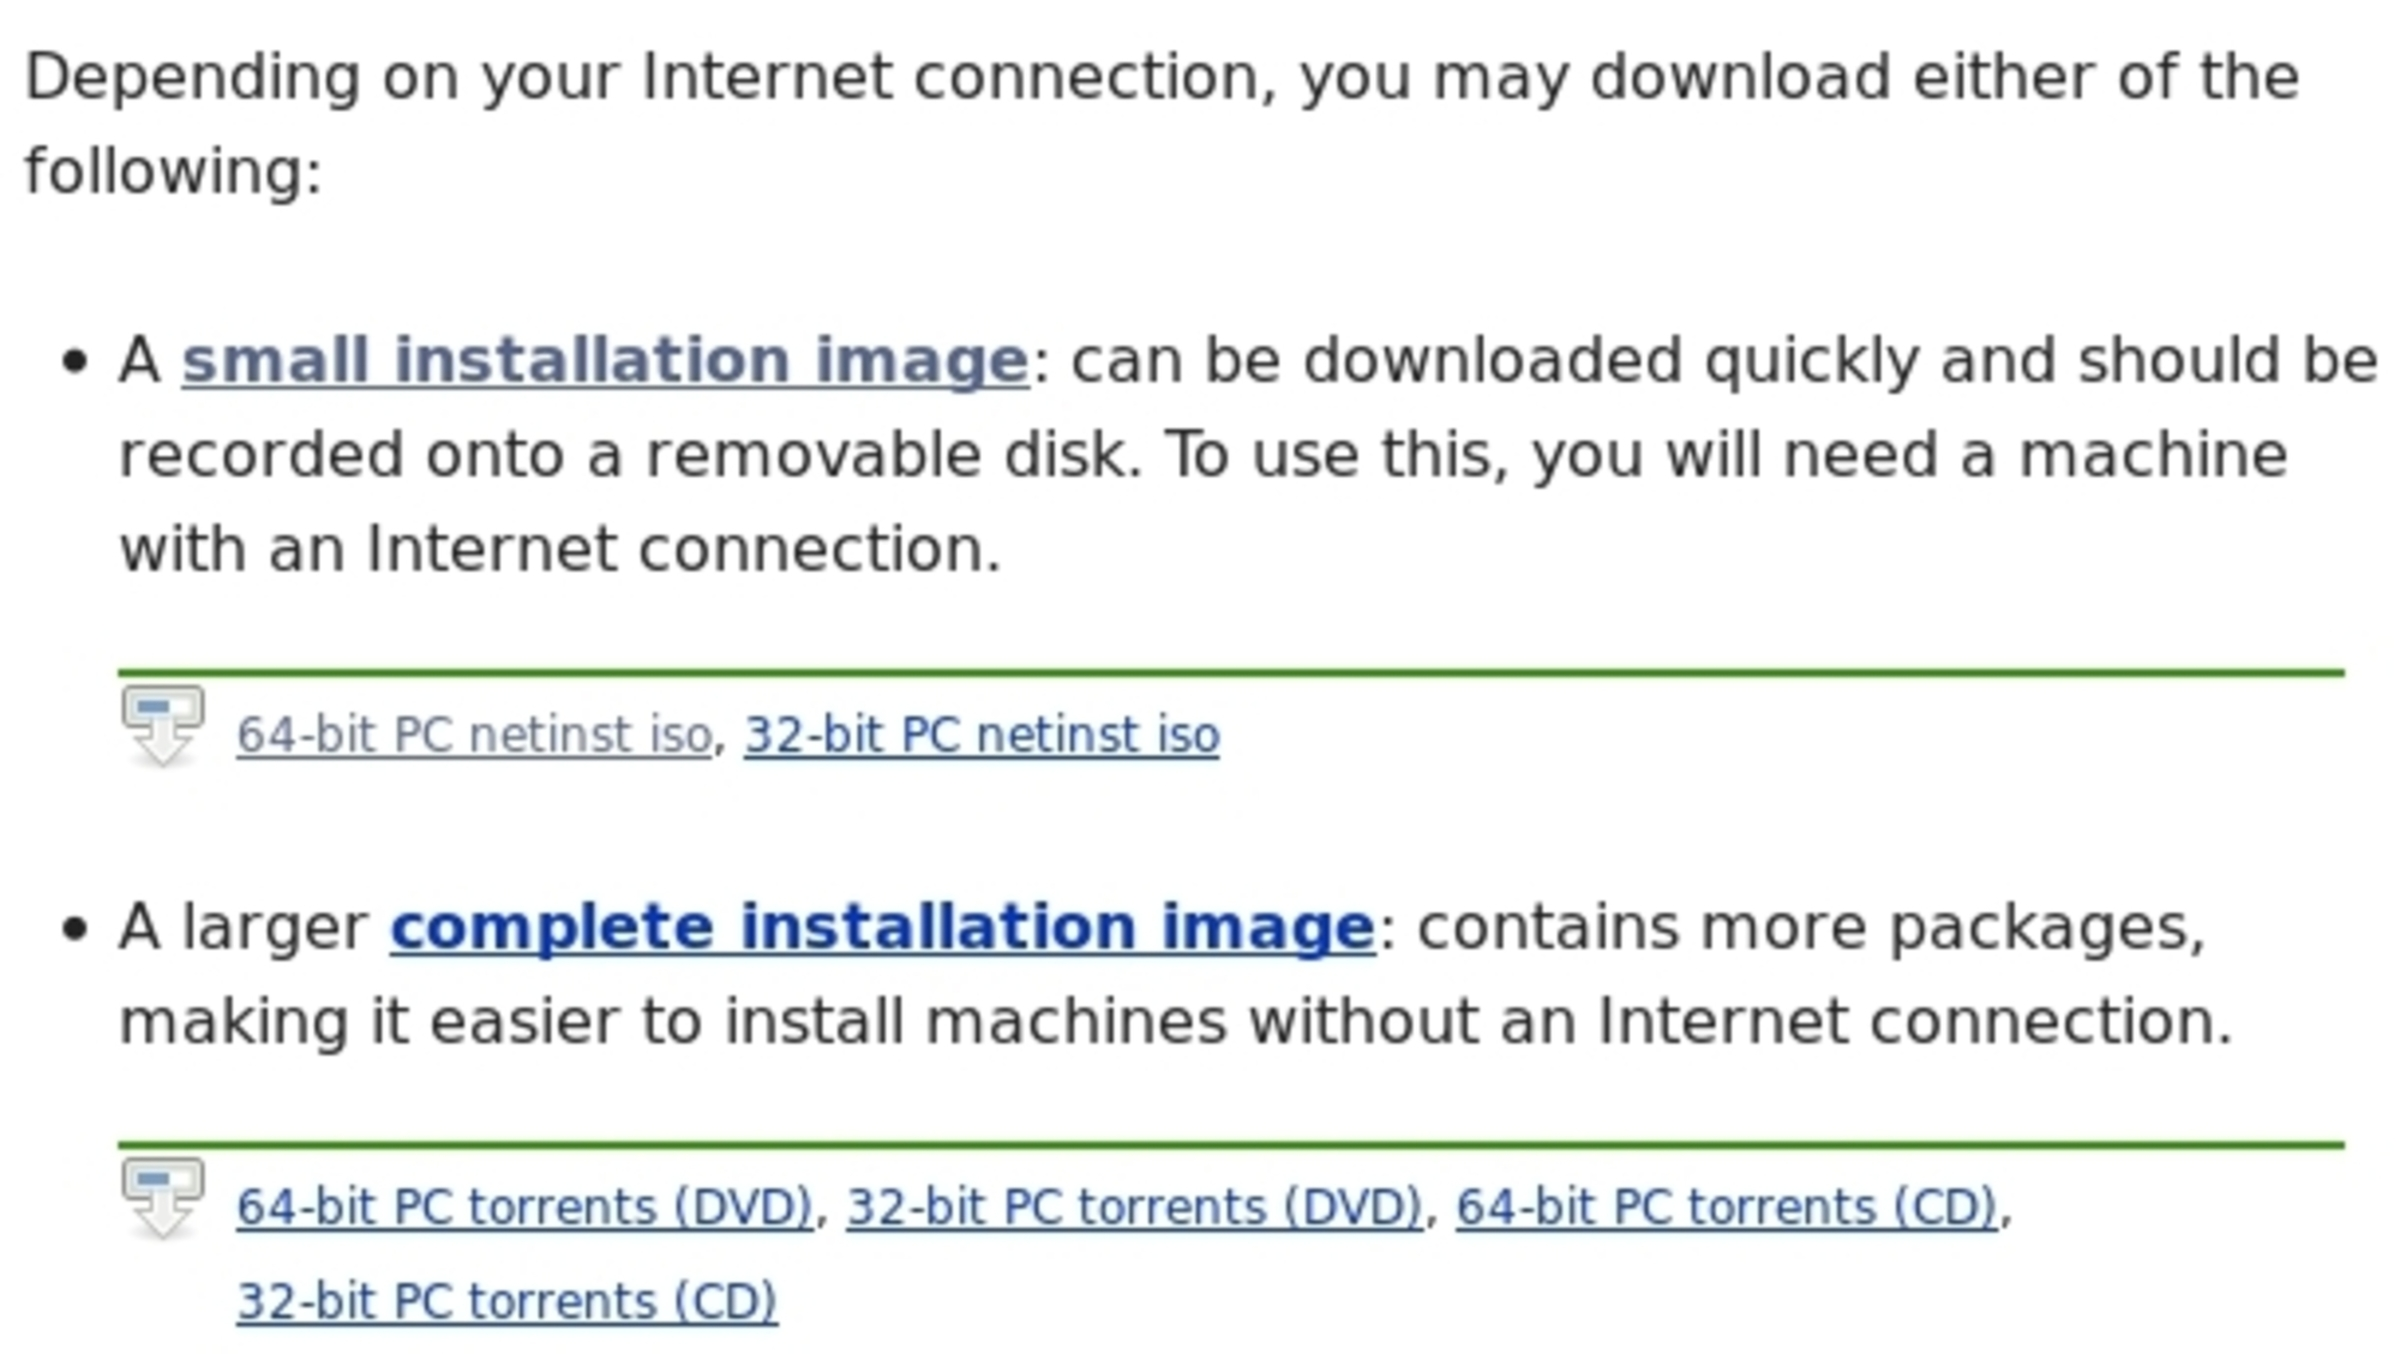
\includegraphics[resolution=600]{get-debian}
	\caption{Pagina di download di Debian}
	\label{fig:get-debian}
\end{figure}

Possiamo scegliere tra due tipi di file immagine: \textit{small (netinst)} e \textit{complete}. Non c'è alcuna differenza tra i due, se non per il fatto che il primo richiede una connessione a internet per l'installazione mentre il secondo no. Il consiglio è di utilizzare la netinst (small) in quanto richiede meno tempo per il download. Dobbiamo però anche scegliere tra due diverse versioni: \textit{64-bit PC amd64} (valida anche per architetture Intel, non inganni il nome) e \textit{32-bit PC i386}. I moderni computer hanno tutti architettura a 64 bit: l'architettura a 32 bit è obsoleta, ma in circolazione sono ancora presenti computer con questa architettura. Per determinare l'architettura del computer da Windows Vista/7 basta seguire alcuni semplici passi: \texttt{Menu Start} > \texttt{Sistema} > click destro su \texttt{Computer} > \texttt{Proprietà} e l'architettura comparirà in mezzo ad altre informazioni. Se il computer è stato acquistato con Windows 8 o successivi, allora sicuramente ha un'architettura a 64 bit; se invece è stato acquistato con Windows XP, allora sicuramente ha un'architettura a 32 bit.

\begin{graybox}
	\textbf{ATTENZIONE:} quanto detto sopra vale solo per computer con architetture Intel o AMD (le più diffuse). Debian però supporta anche altre architetture (ARM, PowerPC, MIPS, e altre ancora). Le immagini per queste architetture speciali, sono disponibili all'indirizzo:

	\texttt{https://www.debian.org/distrib/netinst}
\end{graybox}

Per poter seguire la procedura di installazione descritta nel Capitolo \vref{ch:install}, è necessario scaricare l'\textit{immagine ISO} sul proprio PC.

%&pdflatex
\subsection{Requisiti minimi di sistema}
Per poter installare e poi utilizzare Debian, sono necessari:
\begin{itemize}
	\item Almeno 256 MB di RAM (preferibilmente più di 1 GB);
	\item Almeno 10 GB di spazio su disco rigido (preferibilmente più di 30 GB).
\end{itemize}
In mancanza di questi requisiti, Debian non può essere installato.


%&pdflatex
\section{Prima di cominciare}
Prima di entrare nel vivo dell'installazione di Debian, sono necessarie alcune raccomandazioni.

Intanto si deve decidere se si vuole installare Debian sul proprio computer fisico, oppure se si preferisce utilizzare una \textit{macchina virtuale} (ad esempio con \texttt{qemu} o \texttt{virtualbox}). Nel primo caso, se si possiede già un sistema operativo (come Windows) si deve decidere se si desidera rimpiazzarlo completamente o se si preferisce affiancare l'installazione di Debian a quella dell'altro sistema (\textit{dual-boot}).

Nel seguito, descriveremo un esempio di installazione in dual-boot con Windows 10. Saranno comunque spiegate le (poche) differenze nella procedura per installare Debian come unico sistema operativo. Per quanto riguarda la macchina virtuale, non c'è alcuna difformità rispetto all'installazione fisica e la procedura è identica.

Nel caso di installazione fisica è fortemente consigliato effettuare un \textit{backup} di tutti i propri dati personali su un supporto di archiviazione rimovibile: anche nel caso di installazione in dual-boot. Per l'installazione in macchina virtuale, non c'è alcun rischio di perdita di dati.

